\section{Thrust 3. Predictive Coverage-Guided Intelligent Fuzzing}
\label{sec:thrust3}

\subsection{Framework Overview}
\label{sec:framework}

Fig.~\ref{fig:fuzzwise} shows the overview workflow. The core of {\tool} is a tandem of two Large Language
Models (LLMs): 1) the LLM-based Test Case Generator (TCG), and 2)
CoPilot~\cite{forge24}, the LLM-based coverage predictor. Both
work collaboratively in an iterative fashion in two interleaving
cycles to build the test suite.

First, the LLM-based TCG module examines the source code of the program under
test and generates a number of test cases relevant to a test seed. Initially, the test seed could be given by developers or
automatically generated by the LLM. These test cases are
fed into CodePilot~\cite{forge24} for the estimation of their qualities
with regard to their code coverages. If the new test cases are
estimated to explore the new area (i.e., the total code coverages are
estimated to be higher than the coverage of the current test
suite), they are added to the test
suite. If not, the first loop/cycle (marked with (1) in
Fig.~\ref{fig:fuzzwise}) is continued in which the predicted coverages
are provided as feedback to the TCG for improvement. Our
prompt is designed to instruct and guide the TCG to generate test case(s)
with the goal of covering the not-yet-covered code. The purpose
of this first cycle/loop is to guide the TCG to generate test cases
to explore one potential faulty area in the code.

If CodePilot estimates better cumulative coverage for the
generated test cases, {\tool} engages the second cycle/loop (marked with (2) in
Fig.~\ref{fig:fuzzwise}) after collecting them into the current test suite. With another prompt, it instructs/guides the TCG
to generate more test cases aiming to raise unhandled runtime exceptions
in a different local segment of the source code. The test cases that are
generated in this cycle are fed to CodePilot, for predicting the code coverage.
Finally, the workflow stops when the
time limit is reached.

\subsection{{\tool} Algorithm}




\definecolor{gray}{rgb}{0.5,0.5,0.5}
\definecolor{mauve}{RGB}{127,0,145}
\definecolor{lightgray}{gray}{0.97}
\begin{wrapfigure}{l}{0.5\textwidth}
  \lstset{
    language=Java, caption=, float, morekeywords={do, while, foreach,function,equals,and,or,in}, mathescape=true, escapechar=|,backgroundcolor=\color{lightgray},
	numbersep=-4pt,
	numberstyle=\tiny\color{gray},
	keywordstyle=\color{mauve},
        basicstyle=\scriptsize\sffamily,
	} 
\begin{lstlisting}[caption=]
   $Test\_suite$ = $\emptyset$
   $Cumulative\_cov$ = $\emptyset$
   $Stop$ = False
   $Pred\_cov$ = $\emptyset$
   while (not $Stop$):
      if ($Pred\_cov \cup Cumulative\_cov$ > $Cumulative\_cov$) or ($Cumulative\_cov$ == 100%):
         $T\_seed$, $T\_mutations$[1:$N$] = TCG_LLM($prompt1$)
      else:
         $T\_seed$, $T\_mutations$[1:$N$] = TCG_LLM($prompt2$)
      $Pred\_cov$ = COV_LLM($T\_seed$, $T\_mutations$, $prompt$)
      $Cumulative\_cov$ = update($Cumulative\_cov$, $Pred\_cov$)
      $Test\_suite$.extend($T$_mutations[1:$N$])
      if (time_limit_reached):
         $Stop$ = True
   DuplicationRemoval($Test\_suite$)
   Execute($Test\_suite$)
\end{lstlisting}
\vspace{-6pt}
\caption{FuzzWise Workflow Algorithm}
\label{algo}
\end{wrapfigure}

Listing~\ref{algo} shows the pseudo-code illustrating {\tool}
workflow. It begins by initializing essential variables:
$Test\_suite$ to store generated test cases, $Cumulative\_cov$
to track accumulated coverage of the test suite (starting with an
empty coverage), $Stop$ as a termination flag, and $Pred\_cov$ for
predicting coverage (lines 1--4). The iterative process continues
until a predefined time limit is reached or the test suite reaches the
full coverage of the code (lines 5--14).



The decision-making process within each iteration is dynamic, with
branching based on the evaluation of predicted coverage and the
cumulative coverage. If the predicted code coverage of the newly
generated test cases includes previously uncovered code or the test
suite reaches 100\% coverage on the program (line 6),~we call the
Exception-raising Test Case Generation by invoking the
test-case-generation LLM, $TCG\_LLM$ (line 7),~with the prompt to
guide the LLM to generate test cases aiming to detect runtime
errors/exceptions. If the predict ed code coverage of the new test
cases does not cover the previously uncovered code (line 8), we call
the Coverage-increasing Test Case Generation module by invoking the
test-case-generation LLM, $TCG\_LLM$ with the prompt to instruct it to
generate test cases aiming to increase cumulative code coverage of the
test suite (line 9). These two test generation strategies aim to
produce test cases that target different local vulnerable areas and
subsequently focus on each area to detect unhandled runtime
exceptions. These two strategies are orchestrated using
test-case-generation functions, leveraging LLMs with specific
prompts. Each prompt is designed to instruct the test-case-generation
LLM to generate $T\_seed$ and ($N$) $T\_mutations$, in which $T\_seed$
represents the test seed with potential high coverage, and
$T\_mutations$ are the relevant test cases that cover the similar
areas as $T\_seed$.

After generating $T\_seed$ and $T\_mutations$, {\tool} invokes the
code coverage prediction LLM, CodePilot~\cite{forge24}, on those test
cases (line 10). It then updates the cumulative coverage and extend
the test suite accordingly (lines 11--12). The termination condition,
set to a specified time limit, ensures the algorithm to stop. Upon
conclusion of the loop, we eliminate the duplicate test cases and
execute the generated ones.

%the given program with the generated test suite to identify potential
%runtime errors.

%In instances where the predicted coverage encompasses new statements or the accumulated coverage attains 100\%, the algorithm activates the Exception-raising Test Case Generation utilizing the \textit{EXC-TCG-LLM()} approach. Conversely, when deemed necessary, the algorithm employs the Coverage-increasing Test Case Generation through the \textit{CVG-TCG-LLM()} approach. These mutation strategies are orchestrated by test-case-generation functions, leveraging GPT-based models prompted with specific directives (depicted in Figure 5a and 5b). Both functions yield \textit{T-seed} and \textit{T-mutations}, where \textit{T-seed} represents the test case in the cycle likely to generate the highest coverage or the most effective exception, while \textit{T-mutations} encompass test case mutations that may or may not contribute equally to coverage or error detection.

%Following the generation of test cases (\textit{T-seed} and \textit{T-mutations}), the algorithm incorporates CodePilot to predict the resulting coverage (\textit{Resulting-cov}). The comparison between the resulting coverage and the cumulative coverage informs the decision to update the cumulative coverage and extend the test suite accordingly. The termination condition, contingent on a specified time limit, ensures the algorithm's efficiency, preventing potential computational resource overuse. Upon conclusion of the loop, the algorithm eliminates duplicate test cases and executes a Java program to systematically identify potential Runtime Exceptions.

%The FuzzWise procedure contributes to the field of automated testing by providing an adaptive and dynamic approach to test suite generation. The integration of GPT-based models and CodePilot facilitates an intelligent exploration of test case spaces, optimizing code coverage and potentially uncovering hidden defects in the software under test.

\subsection{Preliminary Results}

{\bf Efficiency in Test Case Generation}. Fig.~\ref{fig:rq2} shows the
test cases generated by {\tool} over the time limit of ten minutes and
the order of the corresponding detected exceptions. The first
exception i.e., \code{Null\-Pointer\-Exception} (Exception 1 on the
y-axis) was found in the first generated test case,
\code{NumberFormatException} (Exception 2 on the y-axis) was revealed
in the 6th test case and
\code{Array\-Index\-Out\-Of\-Bounds\-Exception} (Exception 3 on the
y-axis) was raised in the 20th test case. There are a total of 41 out
of 49 test cases that were effective in detecting one or more runtime
errors/exceptions, in which some of them revealed different instances
of the same exception type.
%
In contrast, Jazzer detected two runtime exceptions. In total, 109,746
test case mutations were generated before the first runtime exception
(i.e., \code{Array\-Index\-Out\-Of\-Bounds\-Exception} was
raised). After this, the second exception,
\code{Number\-Format\-Exception} was raised after 540,202 test case
mutations. Due to the space, we did not show the second one in
Fig.~\ref{fig:rq2}.

%In a period of 10 minutes, in the case of Jazzer, 109746 test case mutations were generated before the first unhandled runtime exception i.e, "ArrayIndexOutOfBoundsException" was raised. After this, the second exception, "NumberFormatException" was raised after 540,202 test case mutations. In the case of {\tool}, the first exception i.e., "NullPointerException" was found in the very first test case mutation, "NumberFormatException" was found in the 14th test case mutation and "ArrayIndexOutOfBoundsException" was raised in the 20th test case mutation.  

\begin{wrapfigure}{l}{0.45\textwidth}
\begin{center}
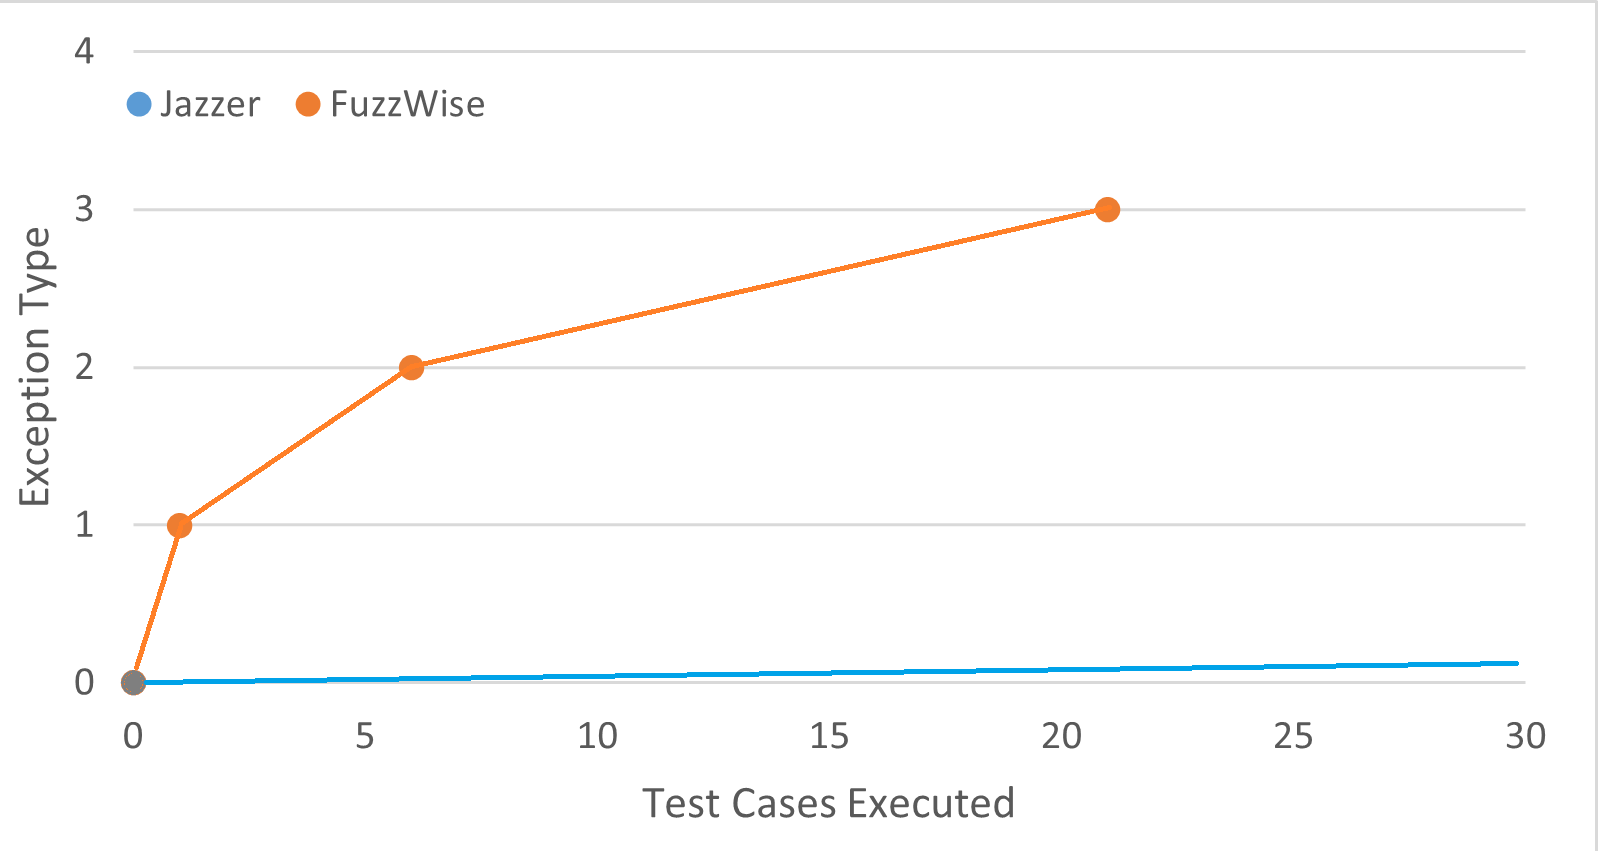
\includegraphics[width=2.6in]{RQ2_exception trend}
\vspace{-9pt}
\caption{Generated Test Cases Revealing Runtime Errors}
\label{fig:rq2}
\end{center}
\end{wrapfigure}

Moreover,  Jazzer generates a total of 18,238,984 test cases to be tested on the code snippet out of which 69,909 (0.38\%) mutations raise an \code{Array\-Index\-Out\-Of\-Bounds\-Exception} and 101872 (0.55\%) test case mutations raise a \code{Number\-Format\-Exception}. In contrast, for the same code snippet and in the same time frame, {\tool} generates a total of 49 test cases out of which 16 of them raised an \code{Array\-Index\-Out\-Of\-Bounds\-Exception},  4 of them raised a \code{NumberFormatException} and 21 raised a \code{Null\-Pointer\-Exception}.
%
Fig.~\ref{fig:rq2} shows ability of {\tool} to quickly
transition to a different local minima, i.e., a different runtime
exception.

%This ability can be attributed to the prompt generating
%architecture of {\tool}, where the coverage increasing prompt and the
%exception raising prompt are set apart from each other. Seperating
%both aspects of test case generation helps {\tool} to increase focus
%and thus reduce hallucination for the LLM over a single local minima.

\subsection*{Avoiding the Coverage Plateau}
\label{sec:rq3}

%\begin{figure}[t]
%\begin{center}
%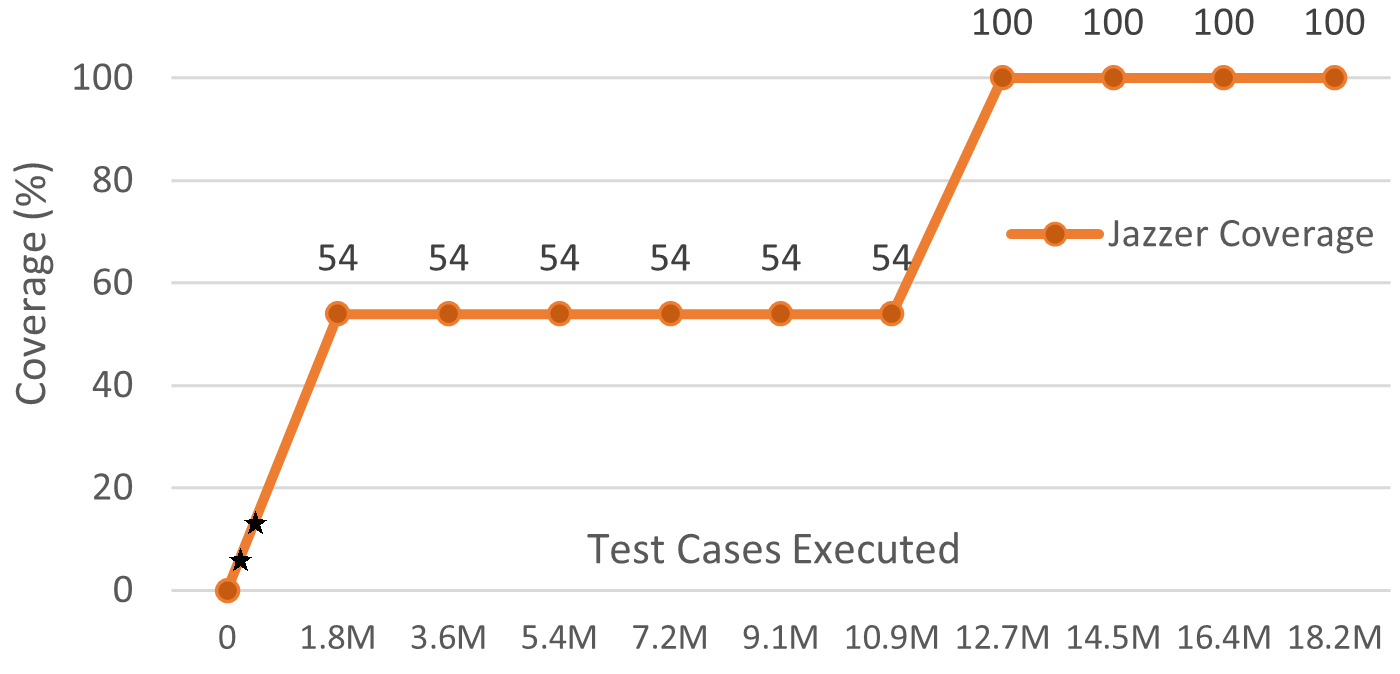
\includegraphics[width=3.5in]{RQ3_jazzer2.png}
%\vspace{-15pt}
%\caption{Coverage trend across the test suite generated by Jazzer (RQ3)}
%\label{fig:rq3-jazzer}
%\end{center}
%\end{figure}

%\begin{figure}[t]
%\begin{center}
%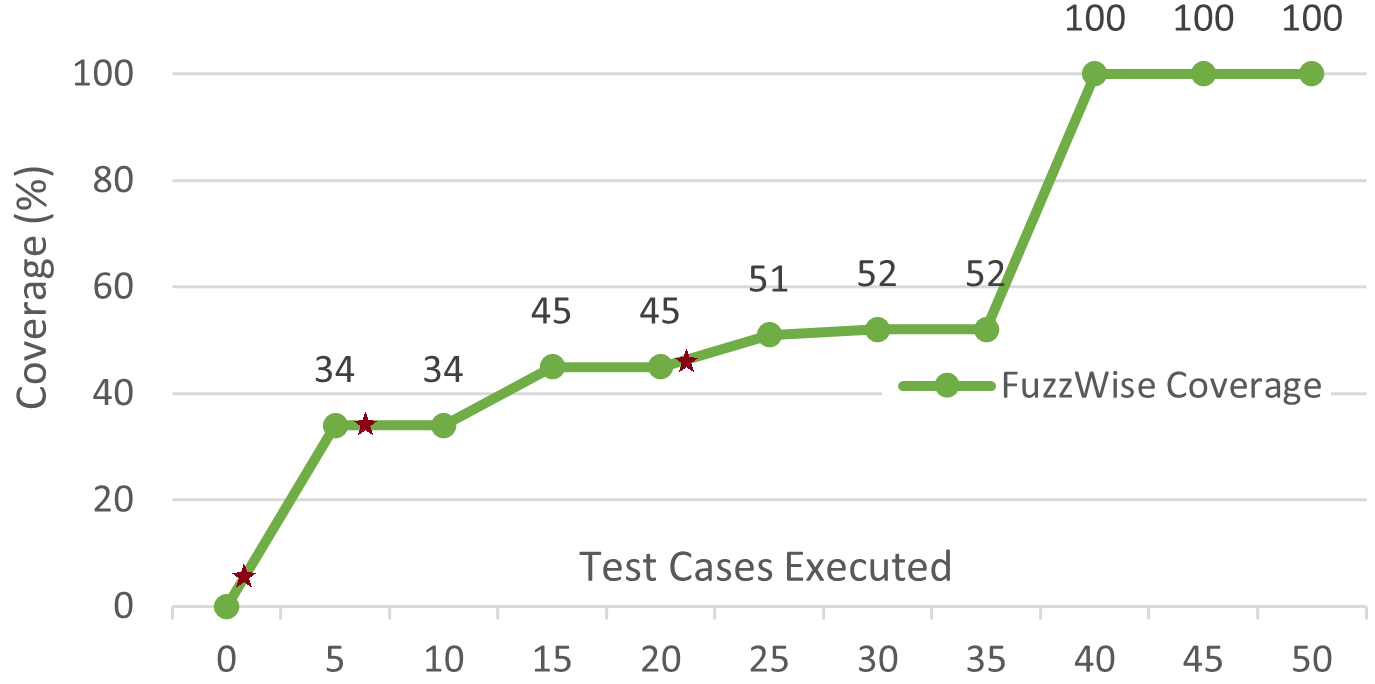
\includegraphics[width=3.5in]{RQ3_fuzzwise2.png}
%\vspace{-15pt}
%\caption{Coverage trend across the test suite generated by {\tool} (RQ3)}
%\label{fig:rq3-fuzzwise}
%\end{center}
%\end{figure}

\begin{figure}[t]
    \centering
    \begin{minipage}{0.5\textwidth}
        \centering
        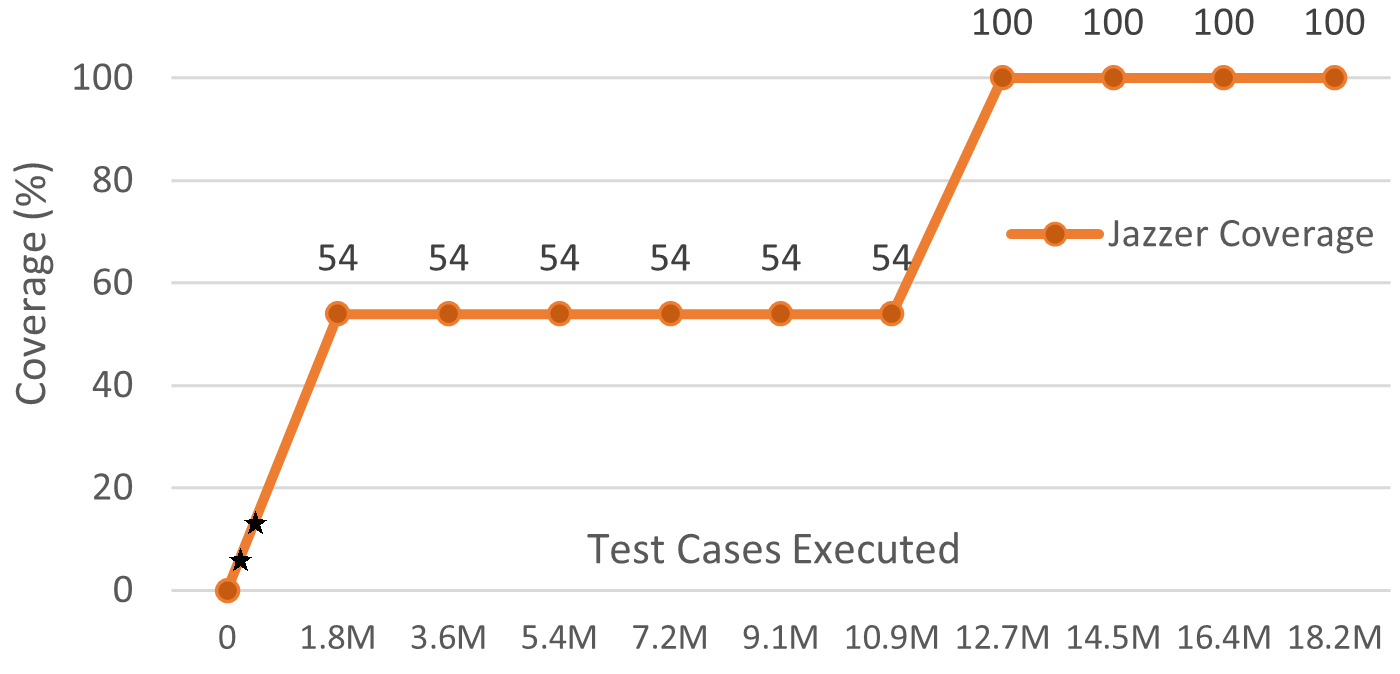
\includegraphics[width=3in]{RQ3_jazzer2.png}
        \vspace{-12pt}
        \caption{Coverage trend across the test suite by Jazzer}
        \label{fig:rq3-jazzer}
    \end{minipage}%
    \begin{minipage}{0.5\textwidth}
        \centering
        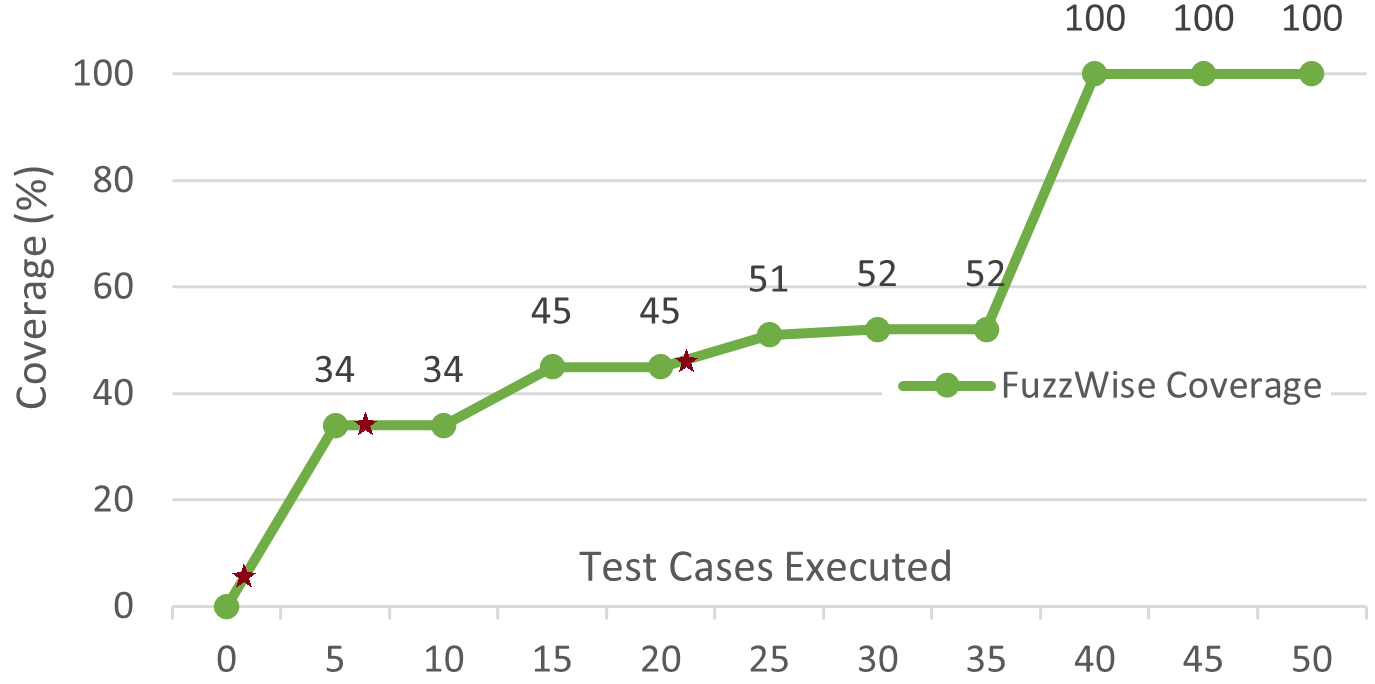
\includegraphics[width=3in]{RQ3_fuzzwise2.png}
        \vspace{-12pt}
        \caption{Coverage trend across the test suite by {\tool}}
        \label{fig:rq3-fuzzwise}
    \end{minipage}
\end{figure}

The coverage plateau issue~\cite{lemieux2023codemosa} encountered by
coverage-guided fuzzers is a scenario where the fuzzing process
reaches a point where further generated test cases fail to
significantly increase the overall code coverage.
%
%This phenomenon might occur when the fuzzer encounters code regions
%that are difficult to trigger or explore.  The coverage plateau issue
%hampers fuzzing effectiveness as it suggests the fuzzer might get
%trapped in a local peak of code coverage, restricting its capacity to
%uncover new bugs or vulnerabilities. Overcoming this plateau is
%essential for improving the efficiency and effectiveness of
%coverage-guided fuzzing techniques.
%
Analyzing the coverage trends for both fuzzers
(Fig.~\ref{fig:rq3-jazzer} and Fig.~\ref{fig:rq3-fuzzwise}) on a code
snippet reveals distinct patterns. In the case of Jazzer
(Fig.~\ref{fig:rq3-jazzer}), a noticeable coverage plateau is observed
within the range of test cases from 1.8M to 10.9M. Jazzer struggles to
surpass the 54\% code coverage threshold for the majority of the test
suite, indicating a limitation in its ability to explore new program
paths effectively. It is noteworthy that the first instances of unique
runtime exceptions occur early in the session, occurring within the
first 200,000 generated test cases (1.11\% of entire test suite).
%generated (as elaborated in RQ2).

Conversely, examining the coverage trend for {\tool}
(Fig.~\ref{fig:rq3-fuzzwise}) reveals an absence of a distinct coverage
plateau until reaching 100\% coverage. This absence is attributed to
the continual enhancement in the quality of test cases generated as
the fuzzing iterations progress, as well as the small degree of test case mutation. {\tool}'s internal feedback loop
dynamically updates the cumulative coverage and incorporates the
latest coverage information into the test case generation prompt. This
feature enables the Large Language Model (LLM) to produce test cases
specifically aimed at covering previously unexplored code segments.
Additionally, it is crucial to highlight that the detection of the
first occurrence of each unhandled runtime exception takes place
within the first 21 generated test suite, specifically at the 1st,
6th, and 21st test case instances. Moreover, {\tool} generates the test suite that reaches full coverage at the 40th test
case, which is significantly sooner than Jazzer (which reaches full coverage
around 13M test cases generated).

%This evaluation reveals {\tool}'s significant advantages over
%traditional coverage-guided fuzzers, particularly in its ability to
%overcome coverage plateaus, leading to better detection of runtime
%exceptions. {\tool}'s dynamic test case generation process,
%facilitated by its internal feedback loop and controlled degree of mutation,
%consistently improves code coverage without encountering stagnation.

%Moreover, the prompt segregation mechanism enhances the quality of test cases, enabling {\tool} to efficiently explore previously uncharted program paths. These findings underscore {\tool}'s potential to significantly enhance the effectiveness and efficiency of fuzzing processes in software testing and security analysis.
